\section{Entwurf}

\subsection{Plattformen}
Für die Entwicklung der Smartphone-App haben wir uns auf die Android-Plattform festgelegt. Bei der Smartwatch-App beschränken wir uns auf die Entwicklung einer Android-Wear-Anwendung. Bezüglich der Beacons verwenden wir ausschließlich Bluetooth LE Beacons, da diese den Low-Energy-Standard erfüllen und somit gut für die Kommunikation mit der Smartwatch geeignet sind.

\subsection{Architektur}
Abbildung \ref{fig:Übersicht} zeigt die wesentlichen Komponenten unseres Systems:

\begin{figure}[H]
\centering
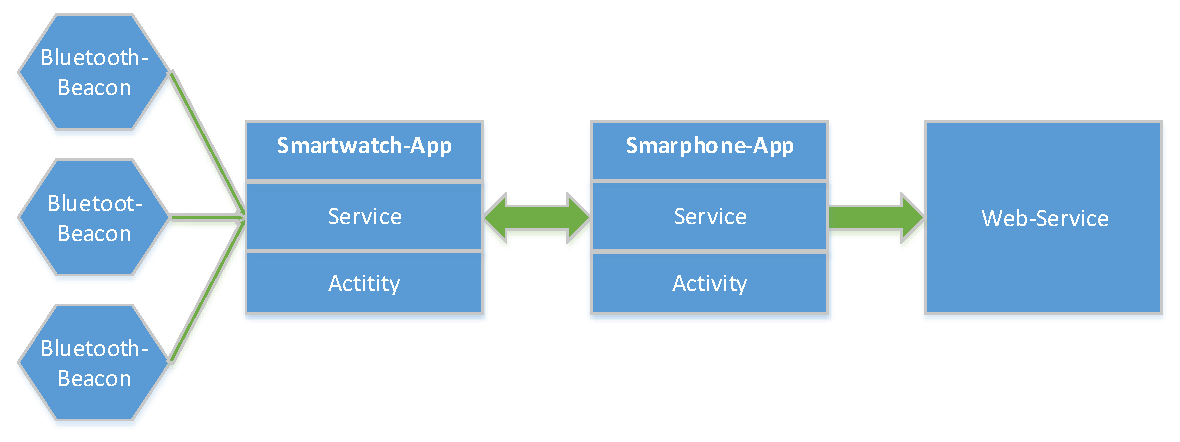
\includegraphics[width=0.95\linewidth]{Bilder/Uebersicht}
\caption{Komponentendiagramm}
\label{fig:Übersicht}
\end{figure}

- Wichtiger Aspekt: Offline-Fähigkeit
Grafik: Komponentendiagramm
Beschreibung des Diagramms und Schnittstellen (ganz grob)

\subsection{Design}

- Usability: Welche Aspekte kann man hier beachten? Keine Eingabe...
\\- Smart Watch hat sehr kleines Display und wenig Eingabemöglichkeiten und unterschiedliche Formen...

Rund und eckig

Kurz ansprechen und auf Details im Folgekapitel verweisen